\chapter{PS board 品質保証試験に向けたコンパクトDAQシステムの開発}
\label{chap_QAQC}

\section{PS board 品質保証試験の設計}
\label{sec_QAQCdesign}
\subsection{PS board 品質保証試験の概要}
\label{subsec_PSBschedule}
2029年から始まる高輝度LHC-ATLAS実験に向けて、TGC検出器エレクトロニクスは刷新される。
フロントエンドエレクトロニクスの1つであるPS boardは、Run 3までのエレクトロニクスに代わり、FPGAを搭載した新しいハードウェアデバイスへと置き換えられる。
図\ref{PSBschedule}にPS boardの量産スケジュールを示す。PS boardはこれまでに第一試作機、第二試作機を用いた機能開発が進められ、2022年にプレ量産が完了している。2024年から1400枚以上に及ぶ本量産が始まり、2026年からATLAS実験室への設置作業が開始される。

% 高輝度LHC-ATLAS実験においても、PS boardはTGC検出器付近に取り付けられたPS-packに設置される。そのため、加速器の運転が始まった後にエレクトロニクスの不具合が発見された場合、修理や交換が困難であり、そのPS board が信号処理を担当する領域は検出器の不感領域となってしまう。

高輝度LHC-ATLAS実験の運転初日から安定したデータ収集を実現するためには、量産された各個体にハードウェアとしての欠陥がないことを詳細に検査することが必要である。そのために行う品質保証試験のことをQuality Assurance and Quality Control (QAQC) 試験と呼ぶ。

本章ではまず、PS board のハードウェアを網羅的に検査することができる試験内容を考案し、それを実現するセットアップを設計した。次に、\ref{chap_TriggerTest}章で述べたシングルボード試験システムの応用として、QAQC試験に向けた試験システムを開発した。最後に、開発したシステムの動作確認とデモンストレーションを行い、PS board QAQC試験に向けたシステム構築を完了させた。

\begin{figure} 
\centering
\includegraphics[width=16cm]{fig/QAQC/PSBschedule.png}
\caption[PS board量産のスケジュール]{PS board量産のスケジュール。これまでに第一試作機、第二試作機を用いた試験が行われ、2022年にプレ量産が完了している。2024年から1400枚以上に及ぶ本量産が始まり、2026年からATLAS実験室への設置作業が開始される。}
\label{PSBschedule}
\end{figure}

\subsection{PS boardに搭載された素子}
\label{subsec_PSBelements}
QAQC試験ではエレクトロニクス上のすべての素子を網羅的に検査し、素子の不良や実装上の欠陥を確実に検出することが求められる。そのために、PS boardに搭載されている素子やそれらの間をつなぐ配線を精査し、試験に適したセットアップおよび試験内容を考案した。

図\ref{PSBconcept}にPS boardに搭載されている素子、各素子間の配線を示す。また、以下にPS board上に搭載されている各素子の役割と各素子間をつなぐ配線をまとめる。

\begin{figure} 
\centering
\includegraphics[width=16cm]{fig/QAQC/PSBoverall.png}
\caption[PS boardの全体像]{PS boardの全体像。PS boardに搭載されている素子とその間の配線を示す。PS boardはSLと3本の光ファイバーで接続され、高速シリアル通信を行う。PS board FPGAから送られる電気信号はSFP+モジュールで光信号へと変換される。また、PS boardはJATHubと2本のCat-6ケーブルで接続される。1本はJTAG線と呼ばれ、JATHubからQSPIフラッシュメモリーにファームウェアを書き込む際に利用される。もう1本はRecovery/Monitor線と呼ばれ、PS board に自己修復不可能なSEUが発生した際のリカバリー手続およびクロックの位相測定に利用される。PS board FPGAとDACは$\mathrm{I^{2}C}$バスで接続され、ADC、Si5395、QSPI、PPASICとはSPIバスで接続される。DACからASDへはアナログの閾値電圧が供給され、ADCはそれをモニターする。PS board FPGAはPP ASICにTTC信号を送信し、ヒット信号を受信する。1つのPP ASICは2台のASDと接続され、それぞれから8チャンネル分のヒットデータを受信する。}
\label{PSBconcept}
\end{figure}

\begin{enumerate}
    \item \texttt{SFP+ :} エレクトロニクス上の電気信号と光ファイバー上の光信号を相互に変換する光トランシーバーモジュール。PS board FPGAは3本の光ファイバーを介してSLと通信する。2本は送信用に定義されており、1枚のPS boardが担当する256チャンネルのヒット信号を送信する。1本は受信用に定義されており、コントロール信号およびTTC信号を受け取る。
    \vskip0.5\baselineskip

    \item \texttt{RJ45コネクター :} Cat-6ケーブルを接続するためのコネクター。JATHubとPS boardは2本のCat-6ケーブルで接続され、LVDS規格で通信する。1本はJTAG線と呼ばれ、JATHubからQSPIフラッシュメモリーにファームウェアを書き込む際に利用される。もう1本はRecovery/Monitor線と呼ばれ、PS board に自己修復不可能なSEUが発生した際のリカバリー手続きおよびLHCバンチ交差クロックの位相測定に利用される。
    \vskip0.5\baselineskip

    \item \texttt{QSPIフラッシュメモリー :} SPIバスによる高速データ転送が可能な不揮発性のメモリー。PS boardではファームウェアおよび制御用パラメーターを保存するのに利用される。ファームウェアはJATHubからJTAG線を操作することで、PS board FPGAを経由して書き込まれる。制御用パラメーターはSLがコントロール信号に乗せてSPIプロトコルをビットバンギングし、PS board FPGAがそれを中継することで書き込まれる。PS board FPGAは自動でこれらのパラメーターを読み出し、PP ASICやDACへ分配する (自律型制御機構)。
    \vskip0.5\baselineskip

    \item \texttt{PP ASIC :} ASDからのヒット信号の処理用に開発されたASIC。可変遅延回路における信号遅延の大きさや、陽子バンチ識別回路の有効ゲート幅はASDごとに異なる値を設定する必要がある。これらのパラメーターは自律型制御機構により、PS board FGPAからSPIバスを通じて設定される。その他に、PS board FPGAからTTC信号やTPT信号を受信し、16 チャンネル分のヒット信号を送信する。PP ASICはASDにテストパルスを供給する。
    \vskip0.5\baselineskip            

    \item \texttt{DAC :} ASDのコンパレーターにアナログの閾値電圧を供給する。PS board FPGAとは$\mathrm{I^{2}C}$バスで接続される。電圧の大きさや極性はASDごとに異なる値を設定する必要があり、自律型制御機構により設定される。設定されたパラメーターは、自律型制御機構により定期的に読み出され、モニター用にSLに送信される。
    \vskip0.5\baselineskip

    \item  \texttt{ADC :} DACからASDに供給される閾値電圧をモニターする。PS board FPGAとはSPIバスで接続される。ADCから読み出された電流のモニター値は自律型制御機構により定期的に読み出され、SLに送信される。
    \vskip0.5\baselineskip

    \item \texttt{Si5395 :} PS board FPGAがシリアルデータから再構成したLHCバンチ交差クロックのジッターを低減し、FPGA、PP ASIC、GTXトランシーバーへ分配する。PS board FPGAとはSPIバスで接続される。Si5395ではクロックの入出力ポートの設定や周波数の設定を行う必要があるが、これらのパラメーターは1434枚のPS boardで共通である。そこで、このパラメーターはQSPIフラッシュメモリーではなく、ファームウェア内のBRAMに固定値として保存される。
    \vskip0.5\baselineskip

\end{enumerate}

\subsection{セットアップおよび試験内容の設計}
\label{subsec_QAQCdesign}
\ref{subsec_PSBelements}節で述べたすべてのインターフェイスと素子を網羅的に検証可能なセットアップとして、JATHubを用いた試験システムを考案した。JATHubはPS boardを試験するための十分なインターフェイスを有していることに加え、拡張性に富んだZynq SoCデバイスをメインドライバーとして搭載している。この特性から、JATHubのPSを起点にすべての試験を完結させる、コンパクトな試験システムを実現できると考えた。図\ref{PSBtestdesign}にその概念図を示す。

\begin{figure} 
\centering
\includegraphics[width=16cm]{fig/QAQC/PSBtestdesign.png}
\caption[PS board QAQC試験セットアップ]{PS board QAQC試験のセットアップ。試験ではPS board 1台に対してJATHub 1台を利用する。JATHubとPS boardは2本のCat-6ケーブルと3本の光ファイバーで接続する。JATHubにPS boardを制御するを実装することで、SLを用いずに試験を完結させる。}
\label{PSBtestdesign}
\end{figure}

このシステムではPS board 1台の試験に、JATHub 1台を用い、JATHubとPS boardを2本のCat-6ケーブルと3本の光ファイバーで接続する。このシステムのコンセプトは、SLが担うPS board 制御機能をJATHubに実装することで、JATHub 1台でPS boardの試験を完結させることである。SLの駆動にはATCAクレートが必要で、大掛かりなセットアップが必要となる。一方、JATHubはデスクトップで給電することも可能であり、場所を選ばない汎用的な試験システムを実現する。以降、QAQC試験のマスター用に開発するJATHubを、QAQC用JATHubと呼ぶ。

QAQC用JATHubのZynq PS領域にはUbuntuを起動する。試験では、ローカルPCからイーサーネット経由でUbuntuにアクセスし、Ubuntu上で実行したアプリケーションを起点に試験用信号の送信や、試験用データの読み出しを行う。Ubuntuは汎用的なOSであり、既存のソフトウェアを用いてネットワークやwebサーバーを構築することができる。また、コンパイラをインストールすることでUbuntu上で直接アプリケーションを作成することができるため、開発を簡単に進めることができる。

FPGA部分であるPL領域には試験用に新しくファームウェアを開発する。
JATHubが担うCat-6ケーブルを介してPS boardを制御する機能 (JTAG線をドライブする機能、リカバリー手続き、クロックの位相測定) に加えて、SLが担う光ファイバーを介してPS boardを制御する機能 (高速光シリアル通信、固定位相でのクロック分配、コントロール信号の送信、固定時間でのヒットデータ読み出し) も実装することで、JATHub1台でPS boardの有する機能を網羅的に試験する。

PS board ハードウェアの動作を網羅的に検証することができる試験として、ASDテストパルス試験とJTAG/Recovery/Clock monitor試験を考案した。以下にそれぞれの試験の概要を示す。

\subsubsection{ASDテストパルス試験}
\vskip0.5\baselineskip
\label{subsubsec_testpulse}
ASDテストパルスは、PP ASICからASDに送られる試験用の電荷であり、ASDからSLまでのデータパスの試験に使用される。高輝度LHC-ATLAS実験のTGCシステムでは、TPT信号を含むTTC信号は、CTPからSLを中継して各フロントエンドエレクトロニクスに分配される。テストパルス生成回路はTPT信号を受信すると、参照クロックである40 MHzクロックの立ち上がりと同期した差動の矩形波をASDに送信する。

% SLにおいて、期待したタイミングにヒット信号得られることを確認することで、ASDからSLまでのトリガーパスにハードウェアの不具合がないこと、およびFixed latencyでのデータ処理を実現できていることを確かめることができる。

PS board QAQC試験ではQAQC用JATHubが試験のマスターとして、PS board を制御する。図\ref{QAQCasdtp}に概要を示す。Zynq SoCのPL領域にPS board制御とヒットデータ読み出し回路を実装し、Ubuntu上のアプリケーションを起点にそれらを制御する。Ubuntuから読み出したヒットデータは、SDカード上にテキストファイルとして保存される。

この試験ではTPT信号を発行してから、固定時間後のヒットビットマップを読み出し、PS board が担当する256チャンネル全てにヒットデータが含まれていることを確認する。これにより、PS boardの制御パスと読み出しパス、およびそれに関係する全ての素子、素子間の導通を検証することができる。具体的には光インターフェイス(SFP+)が正常に動作し光通信が問題なく行われていること。QSPIフラッシュメモリーへのパラメータ書き込みおよびPP ASIC、DAC、Si5395へのパラメータ分配が正常に行われていること。PP ASICによるヒットデータの処理、DACによる閾値電圧の供給、クロックジッタークリーナーによるクロックの分配が正常に動作していること、などを網羅的に検証することができる。以下に具体的な手順について述べる。
% \begin{figure} 
% \centering
% \includegraphics[width=16cm]{fig/QAQC/PSBasdtp.png}
% \caption[ASDテストパルスの概念図]{ASDテストパルス機構の概念図。SLを起点にTPT信号が駆動され、PS board FPGAを経由してPPASICに届けられる。PPASIC内のテストパルス生成はTPT信号を起点に、参照クロックの立ち上がりと同期した試験電荷をASDに送る。ASDで試験電荷はデジタル信号へ変換され、PPASIC、PS board FPGA、SLへとヒット信号が送信される。}
% \label{PSBasdtp}
% \end{figure}

% \begin{figure} 
%     \centering
%     \includegraphics[width=16cm]{fig/QAQC/PSBtpg.png}
%     \caption[テストパルス生成回路]{テストパルス生成回路。PS board FPGAからTPT信号(TRIG)を受け取り、参照クロックである40 MHzクロックの立ち上がりに同期して、ASDに対して差動の矩形波を送信する。}
%     \label{PSBtpg}
% \end{figure}

\begin{figure} 
\centering
\includegraphics[width=16cm]{fig/QAQC/QAQCasdtp.pdf}
\caption[QAQC用JATHubを用いたASDテストパルス試験]{QAQC用JATHubを用いたASDテストパルス試験の概要。QAQC用JATHubが試験のマスターとして、PS boardの制御、TPTの発行、ヒットデータの読み出しを行う。Zynq SoCのPL領域にPS board制御と読み出しのための回路を実装し、Ubuntu上のアプリケーションを起点にTPTの発行およびヒットデータの読み出しを行う。Ubuntuから読み出されたヒットデータは、SDカード上にテキストファイルとして保存される。}
\label{QAQCasdtp}
\end{figure}

\begin{enumerate}
    \item QAQC用JATHubをマスターとして、Ubuntu上のアプリケーションを起点にPS boardに制御パラメーターを設定する。コントロール信号を利用してSPIバスを制御し、PS board上のQSPIフラッシュメモリーにパラメーターを書き込む。その後、PS boardの自律型制御を駆動し、パラメーターをDAC、PP ASICに分配する。PP ASICの制御パラメーターには、ヒット信号遅延、有効ゲート幅、テストパルスの極性、テストパルスの波高、テストバルスの時間幅などが含まれる。
    \vskip0.5\baselineskip

    \item QAQC用JATHubからコントロール信号に乗せてTPTを発行する。また、固定レイテンシー後にL1A信号を発行し、3BC分 (Previous BC、Current BC、Next BC) のヒットデータを読み出す。
    TPTを発行してからヒット信号が返ってくるまでのレイテンシーは、試験セットアップ (シグナルケーブルや光ファイバーの長さなど) に依存する。試験開始前にレイテンシーを測定し、Current BC にヒットが返ってくるよう試験パラメーターを設定する。
    \vskip0.5\baselineskip

    \item TPTの発行とデータ読み出しを複数回繰り返し、読み出したデータにヒットが入っていた割合をEfficiencyとして評価する。PS boardが期待通り動作している場合、Current BC のEfficiencyが1、Previous BC および Next BC のEfficiencyが0になる。
    \vskip0.5\baselineskip

\end{enumerate}

% ASDテストパルス試験によって検証できる素子と素子間の導通を図\ref{QAQCasdtpelements}に示す。

% \begin{figure} 
% \centering
% \includegraphics[width=16cm]{fig/QAQC/QAQCasdtpelements.png}
% \caption[ASDテストパルス試験で検証できる素子]{ASDテストパルス試験で検証することができる素子。ASDテストパルスを期待通り動作させるにはPP ASIC、DAC、Si5395に適したパラーメーターを分配し、ASD、PP ASIC、PS board FPGA、光リンクが同期して動作する必要がある。s赤枠で示す素子と素子間の配線を。}
% \label{QAQCasdtpelements}
% \end{figure}

\subsubsection{JTAG/Recovery/Clock試験}
\vskip0.5\baselineskip
\label{subsubsec_jtag}
JATHubとのインターフェイスの動作検証のため、JATHubからのファームウェアの書き込み、リカバリー手続き、クロック位相測定が正常に動作することを確認する。以下に各試験の概要を示す。

\paragraph{JTAG試験} \par
JTAG試験はZynqに起動したOSからJTAG線をドライブして、QSPIフラッシュメモリーにファームウェアを書き込む試験である。これにはSerial Vector Format (SVF) playerと呼ばれるアプリケーションを用いる。
SVF playerはSVFファイルと呼ばれる、JTAG4線をドライブするパターンを記述したACSII (テキスト) ファイルを読み込み、PS-PL間チップ通信を利用してJTAG線を操作する。SVFファイルはXilinx社が提供するFPGA開発用ソフトウェア "Vivado" で作成することができ、QAQC用JATHub内のSDカード上に置かれる。

\paragraph{リカバリー試験} \par
%図作る
リカバリー試験はPS boardから擬似的に救難信号を出力させ、一連のリカバリー手続が正常に完了することを確認する。これによりRecovery Request線およびProgram線の導通とファームウェアのリセット機構の動作を検証する。

\paragraph{クロック位相測定試験} \par
クロック位相測定試験では、Monitor線を通じてPS boardが再構成したLHCバンチ交差クロックの位相を測定する。これによりクロック分配線の導通およびSi5395の動作を確認する。先行研究で開発された、JATHub内部でのクロック位相測定の方法を図\ref{JATHubclockmeasure}に示す。JATHub内の水晶発振器から生成した40 MHzクロックを参照クロックとして、その立ち上がりのタイミングでLHCバンチ交差クロックをラッチする。参照クロックを1/56 ns刻みでスキャンしながら、ラッチを繰り返すことでLHCバンチクロックの位相を測定する。

\begin{figure} 
    \centering
    \includegraphics[width=14cm]{fig/QAQC/JATHubclockmasurement.png}
    \caption[JATHubによるクロック位相測定の概念図]{JATHubによるクロック位相測定の概念図\cite{mt_atanaka}。PS board からMonitor線 (MON線) を通じて受信した40 MHzクロックの位相を、JATHub内部の水晶発振器で生成した40 MHzクロックを用いて測定する。参照クロックを1/56 ns刻みでスキャンしながら、立ち上がりのタイミングで40 MHzクロックをラッチすることで位相を測定する。}
    \label{JATHubclockmeasure}
\end{figure}    

\clearpage
\section{コンパクトDAQシステムの機能開発}
\label{sec_QAQC_JATHub}
本節では\ref{subsec_QAQCdesign}節で考案した試験を実現するために開発した、QAQC用JATHubの機能実装について述べる。
システムの全体像を図\ref{}に示す。本システムは大きく分けて3つの機能に分けられる。

\begin{figure} 
\centering
\includegraphics[width=16cm]{fig/QAQC/QAQCoverall.pdf}
\caption[コンパクトDAQシステムの全体像]{コンパクトDAQシステムの全体像。本システムは大別して、インフラ機能(図中オレンジ色)、ASDテストパルス試験のための機能(図中み)、JTAG/Recovery/Clock試験機能(図中青色)の3つの機能に分けられる。PS 領域にはUbuntuを起動し、アプリケーションを起点にFPGAを操作する。UbuntuからFPGAの操作はAXI GPIOを利用し、読み出しには自作調停回路を用いる。TTC信号もJATHub内部で生成しPS boardへ分配する。ASDテストパルス試験のための機能は、高速光シリアル通信、PS board への制御信号の送信、固定時間でのヒットデータ読み出しで構成される。JTAG/Recovery/Clock試験に向けて、SVF player、リカバリー手続、クロック位相測定を実装する。}
\label{fig_CTA}
\end{figure}

1つ目はQAQC用JATHub単体でPS board制御およびDAQを完結させるためのインフラの実装である(図中オレンジ色)。Zynq のPS領域にはUbuntuを起動し、LANケーブルを介したEthernet通信を行う。ASDテストパルス試験とJTAG/Recovery/Clock試験はいずれもUbuntu上のアプリケーションを起点に実行する。そのためにUbuntuからFPGAを操作する機能、FPGAからUbuntuへデータを読み出す機能をそれぞれ実装する。QAQC試験ではJATHubをマスターとして、PS board、ASDのタイミング制御も行うため、JAHTub上の水晶発振器で生成した160 MHzクロックを分周した40 MHzクロックをLHCバンチ交差クロックの代わりに、基準クロックとして利用する。またそれぞれのシステムのタイミングを制御するTTC信号もこれを元にJATHub上で生成する。

2つ目はASDテストパルス試験のための実装で、基本的にはSLが担う機能を模したものである(図中緑色)。これにはPS boardとの高速光シリアル通信、固定位相でのクロック分配、PS board への制御信号の送信、固定時間でのヒットデータ読み出しが含まれる。

3つ目はJTAG/Recovery/Clock試験のための実装で、本番運用でのJATHubの担う機能である(図中青色)。これにはSVF player、リカバリー手続、クロック位相測定が含まれる。本研究に取り組んだ2022年当時、高輝度LHC-ATLAS実験用のSLは開発段階にあったため、ASDテストパルス試験のための機能実装はRun3のSLを参考にした。JTAG/Recovery/Clock試験のための機能実装は、先行研究\cite{mt_atanaka}により機能開発が完了していたため、それをそのまま実装した。以下にそれぞれの機能実装について述べる。

\subsection{インフラの実装}
\label{subsec_infra}

\subsubsection{Zynq PS領域におけるUbuntuの起動}
\vskip0.5\baselineskip
\label{subsubsec_ubuntu}
Zynq SoCのPS領域には標準的なLinux OSであるUbuntuを起動する。Ubuntuは汎用性と拡張性に富んだOSで、ネットワークの設定やQAQC用JATHub内部でのアプリケーション開発を容易に行うことができる。

Zynq組み込みデザインの開発には64 bit Ubuntu 18.04.6 を用いた。Zynq PL領域に構築する自作論理回路の開発やPS領域のIO設計は、Xilinx社が提供する ”Vivado 2020.2” を利用した。Zynq PS 領域で走るLinuxの設定はXilinx社が提供するクロスコンパイラー ”Petalinux 2020.2” を利用した。PetalinuxではVivadoで生成したハードウェア記述ファイルを元にデバイスツリーやRoot File System (rootfs) を設定することで、Zynqの起動に必要なブートファイルを作成することができる。

QAQC用JATHubではUbuntuの起動にSDカードを利用する。SDカードには2つのパーティション\footnote{ブートファイル用のパーティションはfat32、Ubuntuのrootfs用のパーティションはext4で展開する。}を用意し、Zynqの起動に必要なブートファイルとUbuntuのルートファイルシステムをそれぞれ展開する。図\ref{JATHubboot}にZynq上でのUbuntu起動の流れを示す。JATHubに電源を投入すると以下のシークエンスでUbuntuが起動する。

\begin{figure} 
\centering
\includegraphics[width=12cm]{fig/QAQC/JATHubboot.pdf}
\caption[Ubuntuの起動シークエンス]{Ubuntuの起動シークエンス\cite{mt_okazaki}。JATHubに電源を投入すると、まずFSBLがロードされ、ファームウェアのビットストリームがPL領域に書き込まれる。次にPS領域にLinuxを起動するため、u-bootが起動し、デバイスツリー、カーネルイメージ、Ubuntuのルートファイルシステムがロードされる。}
\label{JATHubboot}
\end{figure}

\begin{enumerate}
    \item First Stage Boot Loader(FSBL)がロードされる
    \item ファームウェアのビットストリームがSoCのPL領域に書き込まれる
    \item LinuxカーネルやOSを起動するためのブートローダーであるu-bootがロードされ、制御が移行される。
    \item u-boot 制御下でデバイスのハードウェア情報を記述したデバイスツリーがロードされる。
    \item u-boot 制御下でLinux kernelがロードされPS領域に構築される。
    \item 制御がLinuxカーネルに移行されLinuxが起動する。
\end{enumerate}

\subsubsection{LANケーブル経由のネットワーク通信}
\vskip0.5\baselineskip
\label{subsubsec_network}
QAQC試験で用いるJATHub試作1号機は図\ref{JATHub_ether}に示す、2通りの方法でEthernet通信を行うことができる。1つ目はLANケーブルを使用するもので、回路上に搭載されたPHY chip (Micrel PHY Chip) を利用して、Ethernet信号をCPUが扱える信号に変換する。2つ目は光ファイバーを用いる方法で、GTXトランシーバーで受けた光信号を1000BASE X PCS/PMAと呼ばれるIPブロックを利用して処理する。QAQC用JATHubでは3本の光ファイバーはPS board との通信に利用するため、LANケーブルを用いる方法を採用する。

\begin{figure} 
\centering
\includegraphics[width=16cm]{fig/QAQC/JATHub_ether.pdf}
\caption[光Ethernet通信の仕組み]{光Ethernet通信の仕組み\cite{mt_atanaka}。QAQC試験で用いるJATHub試作1号機は光を介した方法とLANケーブルを介した方法の2種類でEthernet通信を行うことができる。QAQC用JATHubでは光ファイバーをPS boardとの通信用に使用するため、LANケーブルを用いた方法を採用する。}
\label{JATHub_ether}
\end{figure}


\subsubsection{AXI GPIOを用いたPS-PL間通信}
\vskip0.5\baselineskip
\label{subsubsec_axi}
PS領域からPL領域への通信は、汎用入出力インターフェースであるAXI General Purpose Input Output (GPIO) を介して行う。AXI GPIOによって接続されたPLのレジスタには固有の物理アドレスが割り当てられる。
% 割り当てられれた物理アドレスの例を図\ref{JATHuaddress}に示す。
このアドレスはVivadoのAddress Mapで確認することができ、Address Editorにてユーザーが自由に変更することができる。

PSからAXI GPIO レジスタへは少なくとも2通りの方法でアクセスすることができる。1つ目はUbuntuルートファイルシステム内の /dev/memが提供するキャラクターデバイスをアプリケーションから直接開く方法である。/dev/memを介したアクセスではUbuntuが扱うすべての物理アドレスに制限なくアクセスすることができるため、簡単に使用できる。一方、カーネル動作に必要なレジスタにも意図せずアクセスする危険があるため、カーネルを壊す危険性がある。2つ目の方法は特定のAXI GPIOレジスタをUser space I/O (UIO) としてデバイスツリーに登録し、アプリケーションからUIOドライバーを介してアクセスする方法である。この方法ではUIOに登録したアドレス以外へのアクセスは禁止されるため、カーネルを壊す危険なく安全に制御できる。本システムのコントロールパスにおいては、より実装が簡単な /dev/memを用いる方法を採用した。

% \begin{figure} 
% \centering
% \includegraphics[width=10cm]{fig/QAQC/JATHubaddress.png}
% \caption[アドレスマップ]{JATHub PL領域におけるアドレスマップ。AXI GPIOによって接続されたPLのレジスタには固有の物理アドレスが割り当てられる。}
% \label{JATHuaddress}
% \end{figure}

\subsubsection{PLからPSへのデータ読み出し}
\vskip0.5\baselineskip
\label{subsubsec_readout}

% 一般に、ZynqのPL領域からPS領域へ、安定的かつ高速でデータを読み出すには工夫が必要となる。

% ASDテストパルス試験ではJATHubのFPGAで受信したデータを、高速でUbuntuに読み出すことが求められる。これは、FPGAからUbuntuへの読み出しにかかる時間を短縮することができれば、テストパルス試験におけるイベント数を増やすことができ、より精度の高い試験を実現することができるからである。

% JATHubのFPGAは40 MHzクロックに同期して固定レイテンシーで動作しているが、プロセッサー領域を$\mathcal{O}(\mathrm{ns})$で制御し、FPGAと同期してデータを読み出すことは一般に困難である。PS領域から安定かつ高速にデータを読み出すためには工夫が必要となる。

% 一般にSoCのPS領域をFPGAと同期させてZynqのPL領域からPS領域へのデータ読み出しは、究では異なる速度で動作する2つのプロセス間のデータ転送に利用される、

高速かつ安定的にZynq PL領域からPS領域へとデータを読み出すため、本研究では自作調停回路を用いた読み出しシステムを開発した。
図\ref{JATHubarbitor}に実装した読み出しシステムの概要を示す。

\begin{figure} 
\centering
\includegraphics[width=16cm]{fig/QAQC/JATHubarbitator.png}
\caption[PLからPSへのデータ読み出しシステム概要]{PLからPSへのデータ読み出しシステム概要。UbuntuからFPGA内のデータを読み出すために、AXI GPIOレジスタを利用する。FIFOがレジスタのデータを更新するタイミングとUbuntuがレジスタのデータを読み出すタイミングは制御されている必要があり、制御のために調停回路を実装した。調停回路により、1$\sim$6の動作順序が保証され、安定した読み出しが保証される。}
\label{JATHubarbitor}
\end{figure}

データの読み出しシステムは、FIFO (First In First Out) メモリー、AXI GPIO レジスタ、自作調停回路で構成される。
FIFOメモリーは、データを一定の順番で保持するメモリーで、最初に格納されたデータが最初に取り出される。この特性を利用して、FIFOをPL領域からPS領域へデータを読み出す際のバッファーとして動作させる。FPGAから読み出すデータは、FPGA内の動作クロックに同期してFIFOメモリーに書き込まれる。書き込まれたデータは、PS領域に起動したUbuntuの動作するタイミングに合わせて読み出される。しかし、PS領域からFIFOメモリーに直接アクセスする方法はないため、データの受け渡しには、AXI GPIO レジスタを利用する。

AXI GPIO レジスタはFPGA内のFIFOからもUbuntuからも任意のタイミングでアクセスすることができるため、両者の動作タイミングを調整する仕掛けが必要である。例えば、Ubuntuがデータを読み出す前にFIFOがAXI GPIO レジスタのデータを書き換えると、書き換える前のデータはUbuntuから読み出されることなく失われることになる。また、FIFOがデータを書き換える前にUbuntuが2回読み出し動作を行うと、同じデータを重複して読み出すことになる。

すべてのデータを漏れや重複なく読み出すために、FIFOとUbuntuの動作順序を制御するのが自作調停回路である。この回路はUbuntuからもFPGAからも操作することができる1 bitのフラグと、ステートマシンで構成される。フラグはUbuntuとFIFO間の情報伝達に利用し、0をFIFOからの書き込み待ち、1をUbuntuからの読み出し待ちと定義する。調停回路で実現される読み出しシークエンスを図\ref{JATHubarbitation}に示す。Ubuntu側はフラグをモニターし、1であることを確認するとAXI GPIO レジスタの値を読み出し、その後、フラグを1から0に下げる。FPGA上に実装したステートマシンも同時にフラグをモニターし、0であることを確認するとFIFOにデータ更新用のread enable信号を送り、フラグを0から1に上げる。これによりFIFOがAXI GPIO レジスタのデータを更新する動作とUbuntuがレジスタのデータを読み出す動作の順序が保たれ、漏れや重複のない読み出しが実現される。

\begin{figure} 
\centering
\includegraphics[width=16cm]{fig/QAQC/JATHubarbitation.pdf}
\caption[調停回路のシークエンス]{調停回路のシークエンス。Ubuntu側とFPGA上のステートマシン側で共通のフラグを操作・モニターすることで両者がコミュニケーションをとる。フラグは0をFIFOからの書き込み待ち、1をUbuntuからの読み出し待ちと定義する。Ubuntuはフラグをモニターし、1になったらAXI GPIOからデータを読み出し、その後フラグを0に下げる。FPGAの調停回路もフラグをモニターし、0になったらFIFOにread enable信号を送信し、その後フラグを1に上げる。これにより、FIFOがAXI GPIO レジスタのデータを更新する動作とUbuntuがレジスタのデータを読み出す動作の順序が保たれ、漏れや重複のない読み出しが実現される。}
\label{JATHubarbitation}
\end{figure}

作成した読み出しシステムの動作検証や性能評価は\ref{sec_PSboardQAQCdemo}節で行う。また、この読み出しシステムはPL領域からPS領域へのデータ読み出しに複数箇所使われており、汎用読み出しシステムと呼ぶ。


\subsubsection{TTC emulator}
\vskip0.5\baselineskip
ASDテストパルス試験ではJATHub、PS board、ASDの間で固定位相でLHCバンチ交差クロックを分配し、それぞれのエレクトロニクスが同期して動作する必要がある。TGCシステムではLHCバンチ交差クロックはCTPから分配されるが、本試験システムではJATHub 1台で試験を完結させるため、JATHub上の水晶発振器で生成されたクロックを基準クロックとして扱う。Bunch Counter Reset (BCR) 信号やEvent Counter Reset (ECR) などのTTC信号も、JATHub内で生成しPS boardへと分配する。この役割を果たすのがTTC emulatorである。ここで発行されたTTC信号はコントロール信号のワード0に埋め込まれ、光ファイバーを介してPS boardへと送られる。L1A信号もTTC emulatorから出力され、前述したようにTPTとL1Aを同期して制御することでFixed latencyのDAQを実現している。以下にTTC emulatorのサブモジュールを説明する。

\begin{itemize}
    \item {TTC generator : } 40MHz LHCバンチ交差クロックで動作するカウンター。reset信号でカウンターをリセットし、1クロックチック毎にカウンターの値を1つずつインクリメントする。カウンターの値が3564に達したタイミングでBCR信号を発行する。デフォルトの設定ではTPT、L1AもBCRに合わせて3564 BCに一回発行しているが、TPT、L1Aの発行頻度は任意の値に設定することができる。TPT lengthを変更することで、TPTを複数BCに渡って出力することも可能になっている。
    \vskip0.5\baselineskip

    \item{TTC Delay : }1 bit 幅、深さ 4096 列のBRAMで実装したディレイ回路。L1A、BCR、TPTに任意の遅延をかけることができる。L1A Delayを調整することでTPTからL1Aを発行するまでのレイテンシーを変更することができる。
    \vskip0.5\baselineskip

    \item{ID counter : }BCR、ECR、L1Aを受けてBCID、ECID、L1IDを数え上げるカウンター。ここで発行されたBCIDやL1IDはUbuntuからの読み出しフォーマットに組み込まれて出力される。読み出したデータにおけるL1IDの連続性やBCIDを確認することでデータの欠損や重複をチェックすることができる。
    \vskip0.5\baselineskip
    
    \item{FPGAテストパルス発行機能 : }PS boardの持つFPGAテストパルスを発行するためのモジュール。FPGAテストパルスはPS board内のBRAMに保存される。BRAMのaddressを指定した状態で、TPTを発行するとBRAMから256 bitのヒットビットマップが取り出され、ASDからのヒット信号の代わりにJATHubに送信される。
    \vskip0.5\baselineskip
\end{itemize}

\subsection{ASDテストパルス試験のための機能実装}


\subsubsection{コントロール}
\label{subsubsec_control}
QAQC用JATHub上の各機能の制御はControl Centerから行う。Control Centerでは複数のレジスタがインスタンス化されており、このレジスタの値を書き換えることでFPGA内の各機能を制御する。Control Centerの操作はUbuntu上で実行したアプリケーションを起点に行う。
図\ref{JATHubccenter}にUbuntuとControl Centerの接続を示す。

\begin{figure} 
\centering
\includegraphics[width=16cm]{fig/QAQC/JATHubccenter.png}
\caption[JATHubコントロール回路]{JATHubコントロール回路。ZynqのOSからPL領域のControl Center内のレジスタを操作することによりFPGA内の各機能の制御やPS boardへのコントロール信号を制御する。Control Center内のレジスタ操作はInterpreterが仲介する。UbuntuからAXI GPIO を介してアドレスとデータを指定すると、InterpreterはVMEプロトコルに従ってレジスタの書き込みを行う。データの読み出しには自作調停回路を利用する。}
\label{JATHubccenter}
\end{figure}

Control Center内のレジスタ操作は、VMEプロトコルを模倣した独自のプロトコルに従って行い、Interpreterがその操作を仲介する。Zynq PS領域とInterpreterは16 bitのData、12 bitのAddress、読み書きモード選択用のそれぞれ1 bitの信号線で接続される。UbuntuはControl Center内のレジスタアドレスを指定し、read modeまたはwrite modeを1に引き上げることで、レジスタの読み書きを行う。この設計により、PSからControl Center内の各レジスタへ直接AXIバスを接続する必要がなく、PSからPLに伸びるAXIバスの本数を必要最小限にとどめることができる。Control Center からUbuntuへのデータ読み出しは、前述の汎用読み出しシステムを利用する。

\subsubsection{PS boardとの通信}
PS boardの制御はSLとPS board間で定められた通信フォーマット(図\ref{TGC_PSBdownlink})に従って、高速光通信を介して行われる。
QAQC用JATHubにも、このフォーマットに従ったパケット交換を行う機能を実装し、PS boardのコントロールおよびLHCクロックの分配を行う。200 MHzのTXユーザークロックで動作するステートマシンにより、40 MHzおきに5ワードを送信する。

PS boardへ送るソフトリセット信号やTPT信号はControl Center内のレジスタ操作により制御する。PS board FPGA内のレジスタ操作はワード2、ワード3に定義された16 bitのAddress、Command、Dataを用いて実行する。Commandにより書き込み/読み出し動作を決め、AddressでPS board内のレジスタアドレスを指定し、書き込み動作の場合はDataに設定した値を書き込む。


%DACやPP ASIC制御する方法として\ref{subsec_QAQCdesign}節では自律型制御機構を利用するものを述べた。QAQC用JATHubからPS boardを制御する際も、
PS board上のQSPIフラッシュメモリーへのパラメータ書き込みは、ワード1で定義されたSPIバス制御用信号 (CS BitmapおよびSCLK、SDI) を操作することで行う。
PS board FPGAや各素子の状態のモニター値は、自立型制御機構により定期的に読み出される。DACの設定値、ADCの測定値、FGPAの温度、xADCによる供給電圧値などのデータは表\ref{tab:PSBdatatype}に示すフォーマットに従い、6 bitのデータタイプと4 bitのデータに分割され、QAQC用JATHubに送信される。QAQC用JATHubは図\ref{JATHubmonitor}に示すように、分割されたモニターデータを再構成し、Control Center内のレジスタに自動で分配する。これにより、常に最新のモニターデータがControl Center内のレジスタに反映される。

\begin{figure} 
\centering
\includegraphics[width=16cm]{fig/QAQC/JATHubmonitor.png}
\caption[QAQC用JAThubに実装されたモニター機構]{QAQC用JAThubに実装されたモニター機構。PS boardから送られるモニター用データを自動でデコードし、Control Center内のレジスタに格納する。これにより、常に最新のモニターデータがControl Center内のレジスタに反映される。}
\label{JATHubmonitor}
\end{figure}

% \begin{figure} 
% \centering
% \includegraphics[width=10cm]{fig/QAQC/PSBdataformat.png}
% \caption[PS boardから送信されるモニターデータのフォーマット]{PS boardから送信されるモニターデータのフォーマット}
% \label{PSBdataformat}
% \end{figure}

\begin{table}[]
    \centering
    \caption[PS boardから送信されるモニターデータのデータタイプ]{PS boardから送信されるモニターデータのデータタイプ。}
    \label{tab:PSBdatatype}
    \begin{tabular}{|cccccc|l|}
    \hline
    \multicolumn{6}{|c}{Data type {[}5:0{]}}                                                                                       & \multicolumn{1}{|c|}{PS Data {[}7:0{]}} \\ \hline\hline
    \multicolumn{1}{|c}{0} & 0                      & 0                      & 1                      & 0                      & 0 & ADC data {[}15:12{]}                   \\  
    \multicolumn{1}{|c}{0} & 0                      & 0                      & 1                      & 0                      & 1 & ADC data {[}11:8{]}                    \\  
    \multicolumn{1}{|c}{0} & 0                      & 0                      & 1                      & 1                      & 0 & ADC data {[}7:4{]}                     \\  
    \multicolumn{1}{|c}{0} & 0                      & 0                      & 1                      & 1                      & 1 & ADC data {[}3:0{]}                     \\  \hline
    \multicolumn{1}{|c}{0} & 0                      & 1                      & 0                      & 0                      & 0 & DAC data {[}15:12{]}                   \\  
    \multicolumn{1}{|c}{0} & 0                      & 1                      & 0                      & 0                      & 1 & DAC data {[}11:8{]}                    \\  
    \multicolumn{1}{|c}{0} & 0                      & 1                      & 0                      & 1                      & 0 & DAC data {[}7:4{]}                     \\  
    \multicolumn{1}{|c}{0} & 0                      & 1                      & 0                      & 1                      & 1 & DAC data {[}3:0{]}                     \\  \hline
    \multicolumn{1}{|c}{0} & 0                      & 1                      & 1                      & 0                      & 0 & xADC data {[}15:12{]}                  \\  
    \multicolumn{1}{|c}{0} & 0                      & 1                      & 1                      & 0                      & 1 & xADC data {[}11:8{]}                   \\  
    \multicolumn{1}{|c}{0} & 0                      & 1                      & 1                      & 1                      & 0 & xADC data {[}7:4{]}                    \\  
    \multicolumn{1}{|c}{0} & 0                      & 1                      & 1                      & 1                      & 1 & xADC data {[}3:0{]}                    \\  \hline
    \multicolumn{1}{|c}{0} & 1                      & 0                      & 0                      & 0                      & 0 & SEM data {[}15:12{]}                   \\  
    \multicolumn{1}{|c}{0} & 1                      & 0                      & 0                      & 0                      & 1 & SEM data {[}11:8{]}                    \\  
    \multicolumn{1}{|c}{0} & 1                      & 0                      & 0                      & 1                      & 0 & SEM data {[}7:4{]}                     \\  
    \multicolumn{1}{|c}{0} & 1                      & 0                      & 0                      & 1                      & 1 & SEM data {[}3:0{]}                     \\  \hline
    \multicolumn{1}{|c}{0} & 1                      & 0                      & 1                      & 0                      & 0 & Tempurature data {[}15:12{]}           \\  
    \multicolumn{1}{|c}{0} & 1                      & 0                      & 1                      & 0                      & 1 & Tempurature data {[}11:8{]}            \\  
    \multicolumn{1}{|c}{0} & 1                      & 0                      & 1                      & 1                      & 0 & Tempurature data {[}7:4{]}             \\  
    \multicolumn{1}{|c}{0} & 1                      & 0                      & 1                      & 1                      & 1 & Tempurature data {[}3:0{]}             \\  \hline
    \multicolumn{1}{|c}{1} & 1                      & 1                      & 0                      & 0                      & 0 & Register access Address {[}7:4{]}      \\  
    \multicolumn{1}{|c}{1} & 1                      & 1                      & 0                      & 0                      & 1 & Register access Address {[}3:0{]}      \\  \hline
    \multicolumn{1}{|c}{1} & 1                      & 1                      & 1                      & 0                      & 0 & Register access data {[}15:12{]}       \\  
    \multicolumn{1}{|c}{1} & 1                      & 1                      & 1                      & 0                      & 1 & Register access data {[}11:8{]}        \\  
    \multicolumn{1}{|c}{1} & 1                      & 1                      & 1                      & 1                      & 0 & Register access data {[}7:4{]}         \\  
    \multicolumn{1}{|c}{1} & 1                      & 1                      &1                       & 1                      & 1 & Register access data {[}3:0{]}         \\  \hline
    \end{tabular}
    \end{table}

\subsubsection{高速光シリアル通信}
\vskip0.5\baselineskip
\label{subsubsec_gtx}
PS boardとSL間の高速シリアル通信では、適切なBCIDとFixed latency schemeを実現するため、固定位相でのクロック分配および固定時間でのデータ転送が行われる。
QAQC用JATHubにおいてもこれを達成するため、先行研究\cite{mt_aoki}で開発された高速シリアル通信システムを実装する。これにより、JATHubやPS boardにリセットや再コンフィギュレーションを施しても、両者の基準クロック間の位相関係は変わらず一定となる。この結果、ASDテストパルス試験に置いて、TPT信号の発行からヒットデータが返ってくるまでのレイテンシーが一定に保たれることが保証される。図\ref{JATHubgtx}にシステムの概要を示す。

% SL-PS board間の通信では、光ファイバーを介した固定位相のクロック分配が行われる。
% 固定位相のクロック分配とは、LHCバンチ交差クロックとPS boardで再構成されるクロックの位相関係が、電源の再投入や光リンクのリセットで変化しないことを意味する。
% は、PP ASICで適切なBCIDをするのに必要不可欠な要請である。PS boardのこの機能を検証するため、QAQC用JATHubを用いたASDテストパルス試験においても固定位相でのDAQが実現されていることを確認する。

% ASDテストパルス試験では固定レイテンシーでのデータ収集を行うため

\begin{figure} 
\centering
\includegraphics[width=16cm]{fig/QAQC/JATHubgtx.png}
\caption[QAQC用JATHubにおけるGTXトランシーバーの概要]{QAQC用JATHubにおける固定位相でのクロック分配GTXトランシーバーの概要。GTXトランシーバーはJATHub内部の水晶発振器で生成した160 MHzクロックを参照クロックとして利用する。TXユーザーロジックはGTX トランシーバーと同期した200 MHz のTXUSER CLOCKで動作する。RX ロジックでは、PS board から受信したシリアルデータから、固定位相でRXUSER CLOCKを再構成するため、Comma detectorを実装する。これによりJATHubとPS board間におけるデータの送受信が固定時間で行われることが保証される。}
\label{JATHubgtx}
\end{figure}


\paragraph{TXロジック} \par
QAQC用JATHubとPS boardはJATHub上の水晶発振器で生成される160 MHz クロック\footnote{正確にはLHCバンチ交差クロック40.079 MHzの4倍に相当する160.316 MHz。}を基準クロックとして、これと同期して固定時間でデータを送受信する。

TXロジックは160 MHzクロックを200 MHzに分周したものを、動作クロック (TXユーザークロック) として利用する。
TXロジックは、200 MHzおきに32 bitのデータ (1ワード) をGTXトランシーバーに送信する。GTXトランシーバーは8b/10bのプロトコルでこれを40 bitのパラレルデータへとエンコードした後、シリアルデータへと変換する。生成されたシリアルデータは、参照クロックから生成した4 GHz クロックに乗せられ、PS boardに送信される。


\paragraph{RXロジック} \par
QAQC用JATHubのRXロジックでは、Fixed latencyでのデータ受信を実現するため、受信したデータから固定位相でRXの動作クロック (RXユーザークロック) を再構成する必要がある。
その実現に重要な役割を果たすのが、RX Clock Data Recovery機構(CDR)とComma detectorである。CDR機構とは受信したシリアルデータの立ち上がりまたは立ち下がりのタイミングに同期してクロックを再構成する機能で、受信データから固定位相で4 GHz クロックを再構成する。
このクロックを1/20に分周し、200 MHzのRXユーザークロックを作るが、その過程で合計20種類の位相の不定性が生じる。この中から特定の1つの位相を決めるのがComma detectorである。Commaデータとは送信側と受信側の間で事前に取り決められた10 bitの予約語で、PS boardとの通信では40 MHzに1回送信するよう決める。Comma detectorはCommaデータが200 bitのシリアルデータの下位10 bitにくるまで、RX ユーザークロックをシフトする(図\ref{JATHubcomma})。これにより1/20の分周においても不定性なく、RXユーザークロックを再構成することができる。

\begin{figure} 
\centering
\includegraphics[width=16cm]{fig/QAQC/JATHubcomma.png}
\caption[Comma detectorの概要]{Comma detectorの概要。Comma detectorはGTXトランシーバーで再構成された200 bitのシリアルデータの下位10 bitがCommaワードと一致するまで、RX SLIDEを打ち続け、RXユーザークロックの位相をシフトさせる。これにより、受信するデータに対して、RXユーザークロックの位相を一位に定めることができる。}
\label{JATHubcomma}
\end{figure}




\subsubsection{固定時間でのヒットデータ読み出し機能}
\label{subsubsec_DAQ}
ヒットデータ読み出し機能は、PS boardから受信するヒットデータをイベントごとにまとめ、Zynq PS領域へと安定的にデータを送る機能である。
QAQC用JATHubは光ファイバーを介して、PS boardから25 nsごとに256 bitのヒット信号を受け取る。ヒットデータとそのデータに割り当てられたイベント情報 (BCID、L1ID) はFPGA上でバッファーされ (L1 Buffer)、L1Aにより取り出される。L1 Bufferから取り出された1 BC分のデータはFIFOメモリーにダンプされ、CPUの動作する任意のタイミングでデータパスとは非同期に読み出される。

ヒットデータ読み出し機能の全体像を図\ref{JATHubdaq}に示す。
読み出し回路はTTC emulator、L1 Buffer、Derandomizer、Event Builderで構成される。Derandomizerの入力までのデータ処理はRXユーザークロックを基準クロックに行われ、固定レイテンシーで動作することが保証される。Derandomizerの出力以降は、LHCバンチ交差クロックとは非同期でUbuntuの動作速度に応じて、処理される。以下に各モジュールの役割を説明する。

\begin{figure} 
\centering
\includegraphics[width=16cm]{fig/QAQC/JATHubdaq.png}
\caption[読み出し回路の全体像]{読み出し回路の全体像。PS boardから25 nsごとに送られる256 bitのヒット信号は、LHC交差クロックに同期してL1 Bufferに格納される。TTC emulatorはTPT信号から固定レイテンシー後にL1Aを発行し、テストパルスに該当するイベントをL1 Bufferから取り出す。取り出されたデータはDerandomizerに入れられ、CPUの動作する任意のタイミングでデータパスとは非同期に読み出される。}
\label{JATHubdaq}
\end{figure}

\subsubsection{L1 Buffer} 
\vskip0.5\baselineskip
L1 BufferはPS boardから受信した256 bitのヒット信号とECRID、L1ID、BCIDなどのタイミング情報を合わせた432 bitのデータを一時的に保管するためのリングバッファーである。TTC emulatorからL1Aが出されたイベントは後段のDerandomizerに転送され、それ以外のデータはここで捨てられる。25 nsごとに到着するヒット信号は、書き込み用ポインタが指すアドレスに格納される。書き込み用ポインタと読み出し用ポインタはLHCバンチ交差クロックに同期して、1ずつインクリメントする。書き込み用ポインタがBRAMの最後尾まで達した場合、次のクロックチックで再び先頭に戻る。L1 depthによって書き込み用ポインタと読み出し用ポインタのアドレスの差を設定することができ、Bufferの深さを任意の値に設定できる。また、L1Aが発行されてから何BC分のデータを読み出すかをReadoutBCによって設定することができる。デフォルトでは3に設定されており、一回のL1Aに対してPrevious BC、Current BC、Next BCの3バンチ分のデータ読み出す。ReadoutBCで設定されたBC分のデータを読み出している途中に再度L1A信号を受信すると、読み出しエラーを出力する。読み出しエラーが生じた場合、そのL1IDをControl Center内のレジスタに格納し、ユーザーが確認できるようになっている。

\subsubsection{Derandomizer}
\vskip0.5\baselineskip
Derandomizerは、後段で行われる読み出しの処理待ちバッファーであり、432 bitの入力データを32 bitずつ出力する。DerandomizerはFIFOを2つ直列に並べることで実装している。
データの分割にはFIFO IPのスライス機能\footnote{FIFO IPでは入力bit幅の1/2、1/4、1/8のbit幅での出力が可能である。}を利用している。Derandomizerの出力はUbuntuのuint32\_t型と整合性のある32 bitが好ましい。そこで432 bitの入力データに不要な64 bitのデータを加え、512 bitのデータを2つのFIFOで1/4ずつスライスすることで、最終的な出力を32 bitにしている。64 bitの不要データは1つ目のFIFOと2つ目のFIFOの間で捨てられ、Ubunutuからの読み出しには関係しない。

% FIFOは入力されたデータを順番に出力する特性を持ったメモリーである。書き込みと読み出しを非同期に行うことができ、一般にクロックドメインをまたぐデータの送受信に利用される。本システムでは固定レイテンシーで動くFPGA内の読み出し回路とPS領域からのデータ読み出しをつなぐ目的で使用する。
Derandomizerへのデータ書き込みレートがUbuntuからの読み出しレートを上回る場合には、DerandomizerのOccupancyは増大していく。その状態が続くとバッファーのオーバーフローが発生し、データが欠損する。バッファーオバーフローが生じた場合の対応は後に紹介する。

\subsubsection{Event Builder}
\vskip0.5\baselineskip
Event BuilderはDeradomizerに格納された32 bit幅のデータを240 MHzのクロックチック毎に1ワードずつ順番に読み出し、イベントごとに所定のフォーマットに成形する。図\ref{JATHubhitformat}に1イベント分の読み出しフォーマットを示す。PS boardから受信した256 bit $\times$ 3 BC分のデータに加えて、TTC emulator から発行されたTTC信号 (ECRID、L1ID、BCID)およびPSBで発行されたBCIDが含まれる。JATHub内で割り当てられたBCIDとPS boardから返ってきたBCIDの差を確認することで、固定レイテンシーでのデータ通信が実現されていることを確かめることができる。

\begin{figure} 
\centering
\includegraphics[width=16cm]{fig/QAQC/JATHubhitformat.pdf}
\caption[JATHubからのヒットデータ読み出しフォーマット]{JATHubからのヒットデータ読み出しフォーマット。3 BC 分のヒットデータに加えて、デバッグ用にJATHubで付与したBCIDやPS boardで付与したBCIDなどが読み出される。}
\label{JATHubhitformat}
\end{figure}

\subsubsection{読み出し回路の性能}
\vskip0.5\baselineskip
実装した読み出し回路における、読み出しレートの上限を概算することは、QAQC試験を設計するにあたり重要である。例えば、ASDテストパルス試験におけるTPT発行レートはこれにより決められる。Ubuntu上でアプリケーションを実行し、FIFOに格納された1000イベント分のパケットを読み出すのにかかる時間を測定した。
図\ref{JTAHubreadspeed}にその結果を示す。横軸に読み出したパケット数、縦軸に経過時間(s)をとる。得られた測定結果を線形フィットし、その傾きから1パケット読み出すのにかかる時間を概算した。その結果、1イベント分のデータを読み出すのに概ね$85\,\mu\mathrm{s}$かかることがわかった。

\begin{figure} 
\centering
\includegraphics[width=11cm]{fig/QAQC/JATHubreadspeed.pdf}
\caption[PSからのヒットデータ読み出し速度の測定]{PSからのヒットデータ読み出し速度の測定。横軸に読み出したパケット数、縦軸に経過時間(s)をとり、得られた測定結果を線形フィットしている。1イベント分のパケットを読み出すのにかかる時間は85 $\mu\mathrm{s}$程度である。}
\label{JTAHubreadspeed}
\end{figure}

\subsubsection{バッファーオーバーフローへの対応} 
\vskip0.5\baselineskip
万が一、バッファーオーバーフローが生じた場合においてもイベントパケットが崩れることのないよう、Derandomizerにはバックプレッシャー機能を実装した。DerandomizerのOccupancyがあらかじめ設定した容量閾値 (4000/4096) を超えると、L1 Bufferへalmost full信号が送られる。almost full信号を受け取ったL1 Bufferは、処理中のイベントのデータ出力を完遂させたのち (Previousの出力中にalmost full信号が来た場合、Current、Nextのデータまで出力を終えた後)、データの出力を一時的に停止する。Ubuntuからのデータ読み出しが進み、DerandomizerのOccupancyが容量閾値を下回ると、再びデータの出力を再開する。これにより、任意のタイミングで読み出しを開始/終了してもイベントのパケットを崩すことなくデータを読み出すことができる。

\begin{figure} 
\centering
\includegraphics[width=16cm]{fig/QAQC/JATHubbackpressure.png}
\caption[リードアウト回路におけるバックプレッシャー機能]{読み出し回路におけるバックプレッシャー機能。DerandomizerのOccupancyがあらかじめ設定した容量閾値を超えると、L1 Bufferにalmost full信号が送られる。almost full信号を受け取ったDerandomizerは処理中のイベントの出力が終わった後、Derandomizerへのデータ送信を停止する。}
\label{JATHubbackpressure}
\end{figure}


\clearpage
\section{PS board 品質保証試験のデモンストレーション}
\label{sec_PSboardQAQCdemo}

\subsection{試験環境}
\label{subsec_testenv}
東京大学に設置したテストベンチを利用して、開発したQAQC用JATHubの動作検証およびQAQC試験のデモンストレーションを行なった。
セットアップを図\ref{QAQCsetup}に示す。QAQC用のJATHubはVMEクレートに設置し、バックプレーンのJ3コネクターを通じて給電する。PS boardには3.3 Vデジタル電源、3.0 V、-3.0 Vアナログ電源を用意しデスクトップで給電する。QAQC用JATHubとPS boardは3本の光ファイバーと2本のCat-6ケーブルで接続する。1台のPS boardには16台のASDをシグナルケーブルで接続する。

\begin{figure} 
\centering
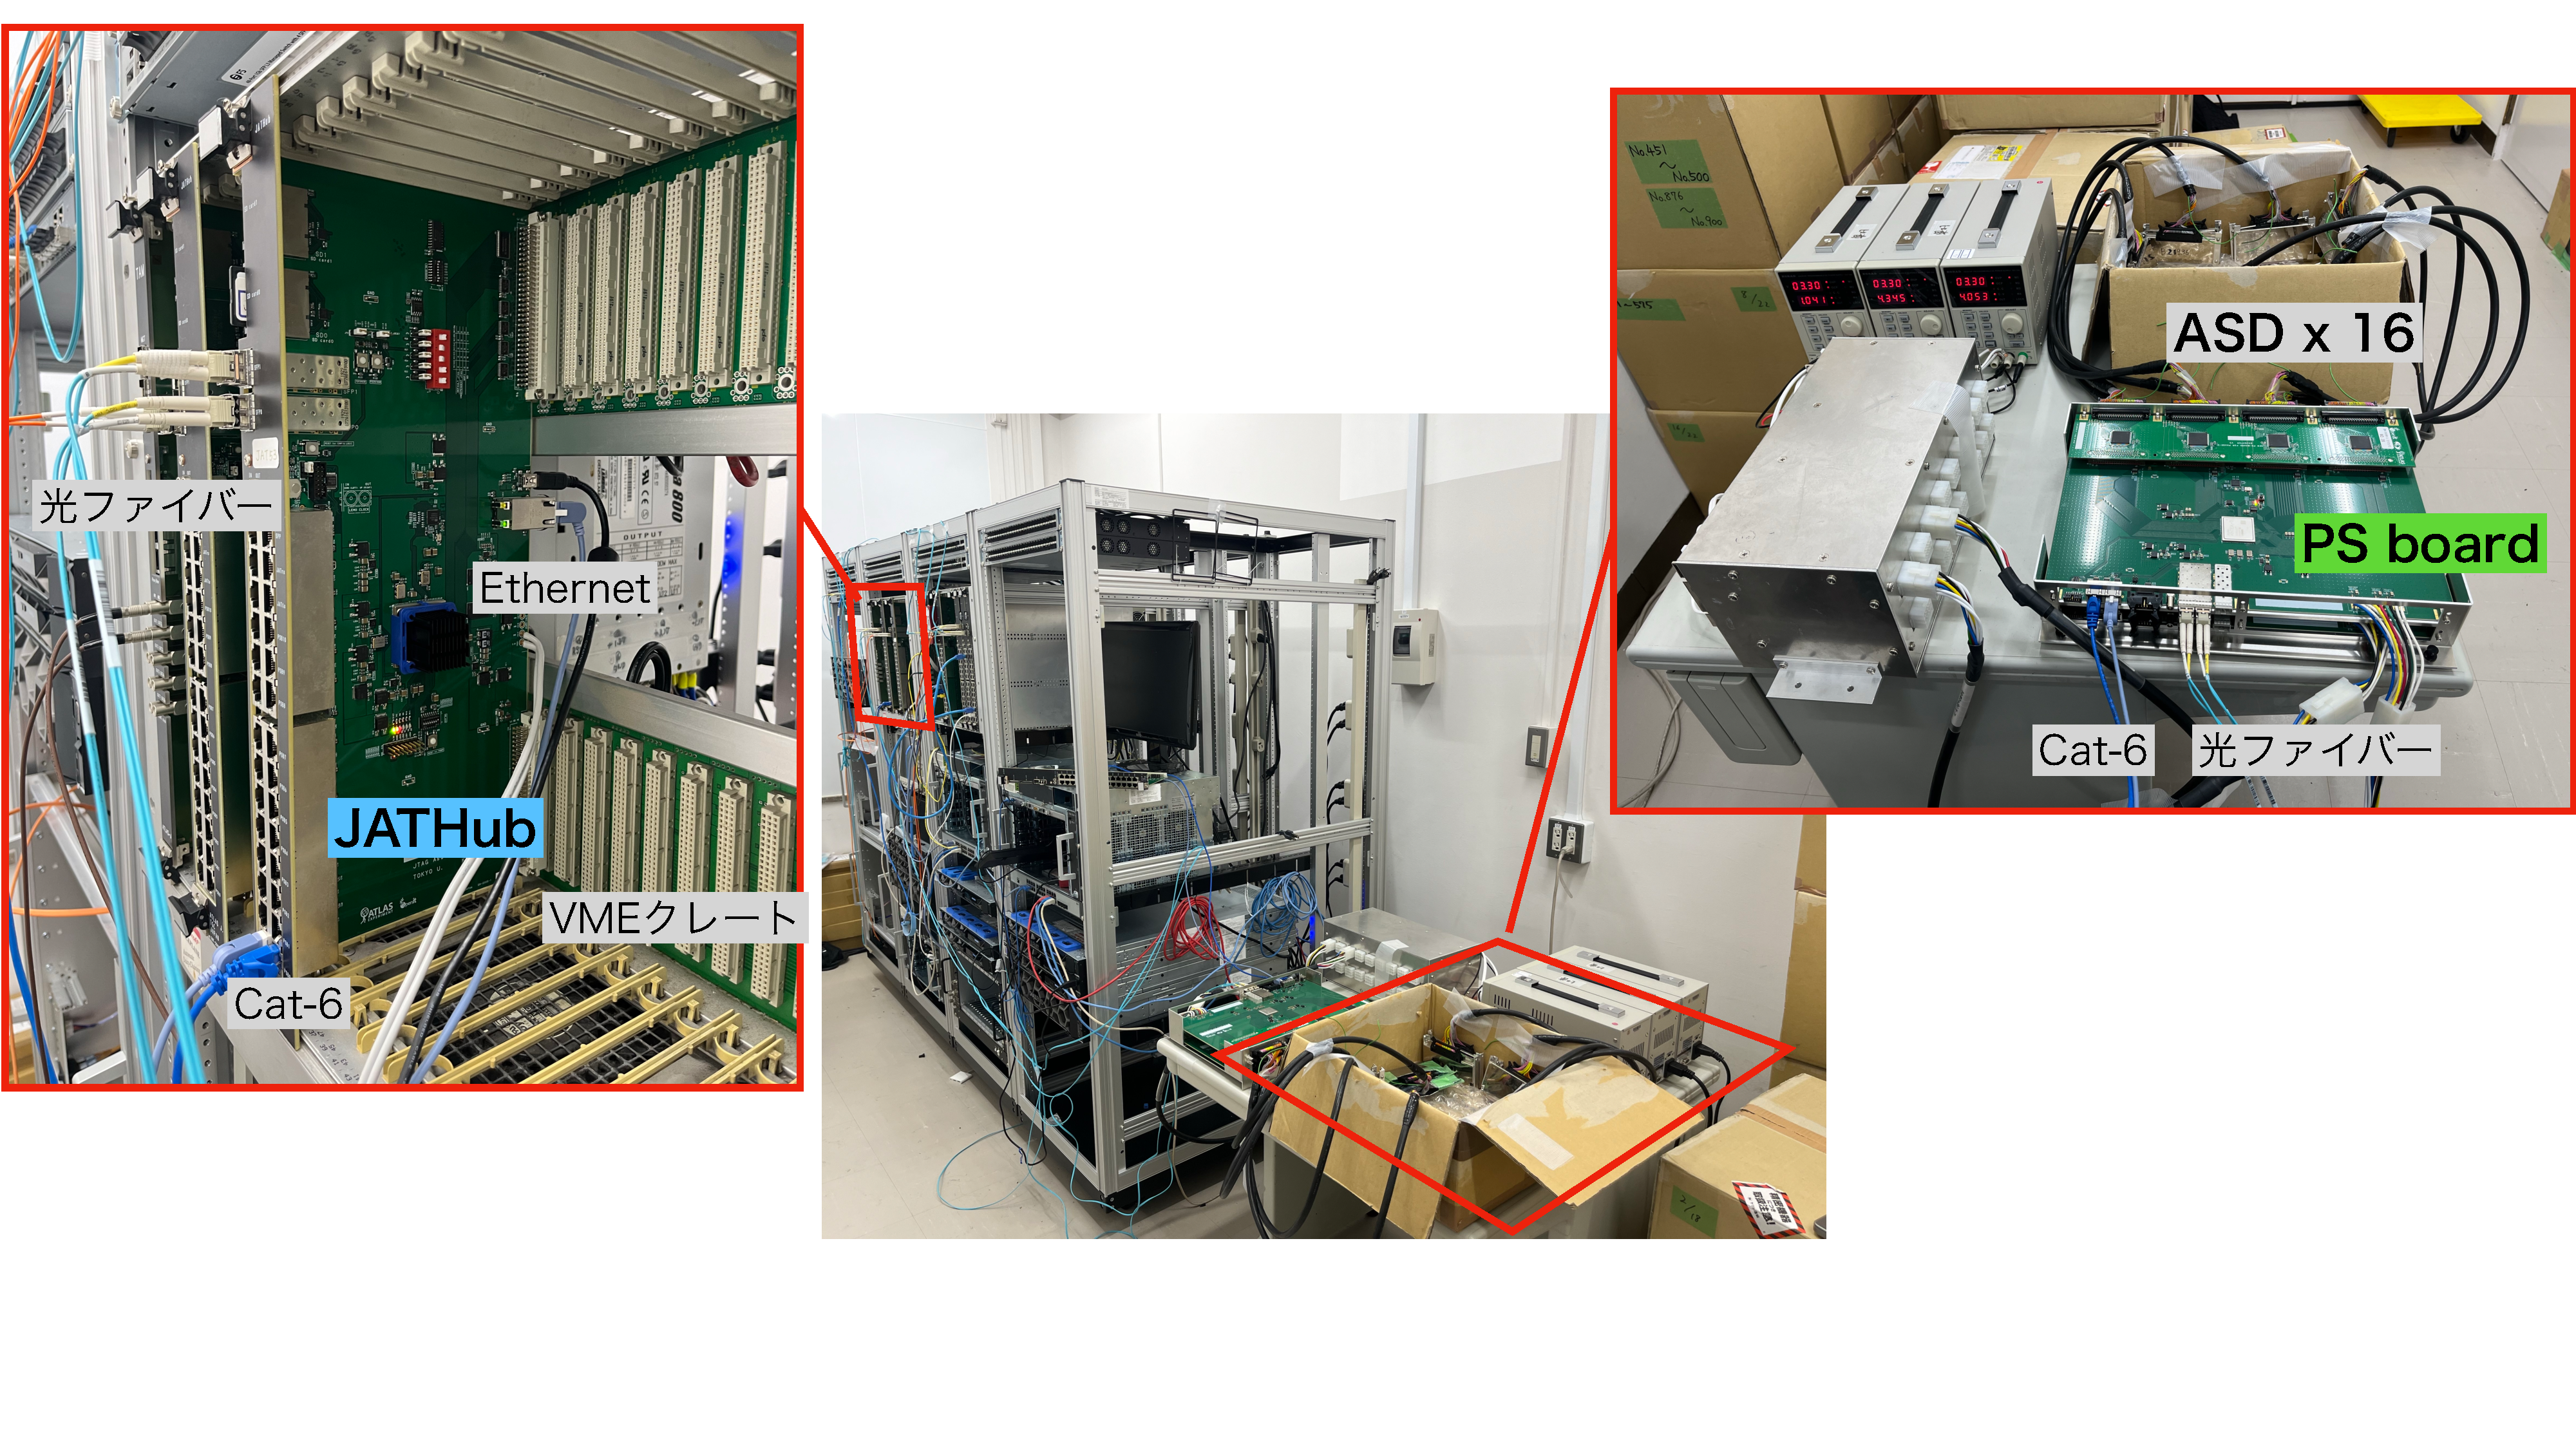
\includegraphics[width=16cm]{fig/QAQC/TB_3goukan.pdf}
\caption[]{QAQC試験のための東京大学でのセットアップ。QAQC用JATHubはVMEクレートに設置し、バックプレーンのJ3コネクターを通じて給電する。PS boardおよびASDには3.3 Vデジタル、3.0 V、-3.0 Vアナログ用電源をそれぞれ用意し、デスクトップで給電する。QAQC用JATHubとPS boardは3本の光ファイバーと2本のCat-6ケーブルで接続する。1台のPS boardには8台のASDを接続する。}
\label{QAQCsetup}
\end{figure}


\subsection{試験用パラメーターの決定とデモンストレーションの結果}
\label{subsec_tb_result}
QAQC試験では量産個体に対する試験に先んじて、PP ASICの遅延、DACの閾値電圧、L1A depthなどセットアップに依存する制御パラメーターを設定しておく必要がある\footnote{ここで決めるパラメーターはQAQC試験を行うためのパラメーターであり、実験時には改めてパラメーターを決めるための調査が行われる。}。
以下に各パラメーターを決定するために行った、事前試験の内容とその結果を示す。

\subsubsection{PP ASIC遅延パラメーター}
\vskip0.5\baselineskip
PP ASICの遅延パラメーターは、使用するシグナルケーブルの長さに依存するパラメーターである。ASDからのテストパルス信号の立ち上がりが、PP ASIC陽子バンチ識別回路におけるLHCバンチ交差クロックの立ち上がりと極めて近い場合、イベントごとに付与されるBCIDが1つに定まらない可能性がある。これを防ぐため、PP ASICの可変遅延回路の遅延パラメーターを変更し、両者の立ち上がりが十分離れるよう調整する。このパラメーターの決定のため、Delayスキャンを行なった。Delayスキャンとは、PP ASICの遅延パラメーターを1 stepずつ変更しながらデータを取得し、付与されたBCIDの変化をみるものである。

あるASDに対するDelay Curveを図\ref{QAQCdelayscan}に示す。横軸に設定した遅延の大きさ、縦軸にEfficiencyを表す。この測定では、陽子バンチ識別回路の有効ゲート幅を25 ns、可変遅延回路の刻み幅を1.19 nsに設定している。遅延が0 nsの時に付与されるBCIDがPrevious BCになるようJATHub内のL1 Buffer Depthを調整した。遅延パラメーターを変更していくと、ヒット信号に付与されるBCIDが1つずつずれ、付与されるBunch tagがPrevious BC 、Current BC 、 Next BCと遷移していく。
この試験の結果、テストパルスの立ち上がりとPP ASICの陽子バンチ識別回路におけるLHCバンチ交差クロックの立ち上がりが十分に離れるよう、遅延パラメーターを20 nsと決定した。
\begin{figure} 
\centering
\includegraphics[width=16cm]{fig/QAQC/QAQCdelayscan.pdf}
\caption[ディレイカーブ]{テストベンチで測定したDelay Curve。あるASDの 16 チャンネル分をまとめて書いている。陽子バンチ識別回路の有効ゲート幅を 25 ns、可変遅延回路の刻み幅を1.19 nsに設定した。遅延が 0 ns の時に付与されるBCIDがPrevious BC になるようL1 Buffer Depthを調整した。遅延を増やすことで、付与されるBCIDが期待通りPrevious BC 、Current BC、Next BCと遷移することがわかる。}
\label{QAQCdelayscan}
\end{figure}

\subsubsection{ノイズスキャン}
\vskip0.5\baselineskip
DACの閾値電圧は、使用するASDのノイズの大きさに依存して変えるべきパラメーターである。ASDには$\mathcal{O}(10 \,\mathrm{mV})$のノイズが乗っていることが知られており、それよりも閾値電圧を低く設定してしまうと、ノイズをヒット信号として処理してしまう。閾値電圧はノイズの値よりも高く、かつテストパルスの波高より十分低く設定する。

DACの閾値電圧決定のためノイズスキャンを行なった。1台のASDに対する結果を図\ref{QAQCnoisescan}に示す。
ASDに印加する閾値電圧を10 mV ずつ変えていき、ノイズレートを測定した。閾値電圧が10 mV 程度になるとノイズによるヒットが見られるようになり、60 mV 以上の閾値電圧をかけるとノイズは消えた。ノイズレートが最大となる点が0 mVからずれているのは、コンパレーターに- 30 mV程度のオフセットが乗っているためである。この結果から本セットアップでのDAC閾値を$\pm$それぞれ+90 mV、-40 mVと設定した。
\begin{figure} 
\centering
\includegraphics[width=16cm]{fig/QAQC/noise_A2.pdf}
\caption[ノイズスキャンの結果]{ノイズスキャンの結果。ASD に印加する閾値電圧を変えながら、10,000 回のテストパルスに対するノイズレートを測定した。ここでは16台あるASDのうちの1台の結果を示している。閾値電圧が -10 mV から 60 mV の間でノイズによるヒットが見られた。}
\label{QAQCnoisescan}
\end{figure}

\subsubsection{デモンストレーションの結果}
\vskip0.5\baselineskip
これらのパラメーターをもとにASDテストパルス試験を行なった。結果を図\ref{QAQCresult}示す。パラメーターを固定した状態で、10,000回テストパルスを発行し、Previous BC、Current BC、Next BCそれぞれのEfficiencyを測定した。結果は、期待通り、すべてのチャンネルでCurrent BCのEfficiencyのみが1となっており、PS board上の各種パラメーターの設定が正常に完了していること、また固定レイテンシーでのDAQが実現できていることを確認した。

\begin{figure} 
\centering
\includegraphics[width=16cm]{fig/QAQC/QAQCresult.pdf}
\caption[ASDテストパルスの結果]{ASDテストパルス試験の結果。10,000回のテストパルスに対する各チャンネルのEfficiencyをプロット。PS board が担う全256チャンネルでCurrent BCのEfficiencyが1であり、Previous BC、Next BC のEfficiencyは0である。このことからASDテストパルスの発行から、読み出しまで固定レイテンシーでの動作が実現されていることがわかる。}
\label{QAQCresult}
\end{figure}

JTAG/Recovery/Clock monitor試験についても試験を行い、期待通りの結果が得られた。これにより、QAQC用JATHubシステムの実装が精度良く達成されていることを確認した。表\ref{table_testtime}に各試験の所要時間を示す。

\begin{table}[]
    \centering
    \caption{各試験にかかる所要時間}
    \label{table_testtime}    
    \begin{tabular}{ll}
    \hline
    試験項目                          & 所要時間   \\ \hline
    SVFプレイヤーによるQSPIファームウェア書き込み    & 40 min \\
    QSPIパラメーター書き込みおよび読み出し         & 2 min  \\
    リカバリー試験                       & 1 s    \\
    電圧値のモニタリング (ADC、xADC) & 2 s    \\
    Clock位相測定                     & 30 s   \\
    ASDテストパルス試験                   & 10 s  
    \end{tabular}
\end{table}

\subsection{試験並列化のためのシステムアップグレード}
\label{subsec_parallel}
QAQC試験のデモンストレーションにより、1枚のPS boardを試験するのに、合計で40 分以上の時間が必要であることがわかった。1400枚のPS boardに対する試験を効率的に完了させるためには、試験の高速化が求められる。単純にはQAQC用JATHub1台とPS board1台のセットアップを複数用意し、並列に試験を行うことが考えられるが、イーサーネット通信のためのRJコネクターと光通信のためのSFP+コネクターを両方有しているJATHubは、試作段階で作成された1台 (試作1号機) しか存在しない。並列化のためには、工夫が必要となる。

そこで、本研究ではVME通信を利用した並列化システムを考案した。システムのセットアップを図\ref{QAQCpararell}に示す。このシステムのコンセプトは、イーサーネット通信ができる試作1号機をQAQC試験におけるマスター(QAQC master)として利用し、QAQC masterから20台のQAQC用JATHub (QAQC slave) を操作することで、20台のPS boardの並列な試験を実現することである。試験の際にはQAQC masterのみを操作して、QAQC slaveに対して試験開始の命令や、試験状況の監視を行う。
QAQC masterはTAMボードを\footnote{Mini-Rackに導入されるTGCエレクトロニクスの一つ。異なる1/24セクター間の陽子バンチ交差クロックの位相合わせに用いられる。}中継して、QAQC slaveと通信する。QAQC masterとTAMは光ファイバーを介したシリアル通信を行い、TAMとQAQC slaveはVME通信を行う。

\begin{figure} 
    \centering
    \includegraphics[width=16cm]{fig/QAQC/QAQCpararell.pdf}
    \caption[並列化システムの概要]{QAQC試験並列化システムの概要。JATHub1台 (QAQC slave) とPS board1台を用いた試験システムを20個並列に設置する。20台のJATHubの動作を制御するため、1台の検査マスターJATHub (QAQC master) を用意する。QAQC masterとQAQC slaveの通信はTAMを介して行う。QAQC masterとTAMは光ファイバーで接続し、高速光通信を行う。TAMとQAQC slaveはVMEバックプレーンで接続され、VME通信を行う。}
    \label{QAQCpararell}
\end{figure}

QAQC slaveにはネットワークが通じていないため、slaveの操作はmasterからのレジスタ操作で行う。QAQC slaveのUbuntuには起動と同時に試験用アプリケーションが走るよう設定し、masterからの合図を起点に1台のPS boardに対する試験を開始する。各試験の結果は2 bitのstatus bitで表され、QAQC masterはそれを読み出すことで各slaveにおける試験の進行状況を把握する。

並列化システムについても、東京大学でテストベンチを構築した。図\ref{QAQCpararellpicture}にセットアップを示す。QAQC master、TAM、QAQC用 slave1台、PS board1台、ASD 16台を接続して、並列化システムの動作検証を行った。QAQC masterの試験開始から、試験の終了まで問題なく動作することを確認した。

% \begin{figure} 
% \centering
% \includegraphics[width=12cm]{fig/QAQC/QAQC_monitor.png}
% \caption[JATHub masterからの試験状況のモニター]{JATHub masterから試験状況をモニターしている様子。QAQCマスターの slaveとして動作する20台のJATHubの試験状況をマスターから把握することができる。この写真はQAQC用 slave1台を用いた試験の際に取られたものであり、JATHub4がそれに該当する。}
% \label{QAQC_monitor}
% \end{figure}

\begin{figure} 
\centering
\includegraphics[width=16cm]{fig/QAQC/QAQCpararellpicture.pdf}
\caption[並列化システムのセットアップ]{並列化システムのセットアップ。QAQC master、QAQC slave、TAMがVMEクレートに設置されている。QAQC masterとTAMは光ファイバーで接続し、QAQC slaveとTAMはVMEバックプレーンで接続されている。QAQC slaveとPS boardは光ファイバーとCat-6ケーブルで接続されている。}
\label{QAQCpararellpicture}
\end{figure}

\section{コンパクトDAQシステムとしての応用例}
\label{sec_compactdaq}
最後に、本研究で開発したQAQC用JATHubのその他の利用例について紹介する。本システムは、Linuxを搭載しており拡張性に富んでいることに加え、デスクトップでも給電可能なコンパクトなシステムである。その柔軟性と利便性から汎用的なDAQシステムとして、TGC検出器の性能評価やエレクトロニクスの試験などに幅広く利用されている。

実際の使用例を2つ紹介する。1つ目はTGC EIL4チェンバーの性能評価である。セットアップを図\ref{JATHubEIL4}に示す。この試験は、高輝度LHC-ATLAS実験に向けて新しく設置されるTGC EIチェンバーの検査を目的としたもので、チェンバーに取り付けたASDからの信号をPS boardで処理し、QAQC用JATHubから読み出している。ASDテストパルスを用いたノイズレートの測定や、宇宙線ミューオンによるチャンネルごとのefficiency測定が行われた。

\begin{figure}
\centering
\includegraphics[width=16cm]{fig/QAQC/JATHubEIL4.pdf}
\caption[QAQC用JATHubの使用例 : EIL4チェンバー試験]{QAQC用JATHubの使用例 : TGC EIL4チェンバーの性能評価試験\cite{mt_wada}。高輝度LHC-ATLAS実験で新しく導入される、TripletのEIL4チェンバーの性能評価を目的としてCERNで行われた。ASDをEIL4チェンバーに接続し、PS board、QAQC用JATHubを用いて信号処理を行うことで、EIL4チェンバーのチャンネルごとの応答を調べている。ノイズスキャンや宇宙線ミューオンを用いたEfficiency測定が行われた。}
\label{JATHubEIL4}
\end{figure}

2つ目はPS boardの放射線耐性試験である(図\ref{JATHubSEU})。この試験は、ATLAS実験室の実際の放射線環境における、PS boardのSEU発生頻度を測定するものである。UX15に設置したPS boardから送られるモニターデータの読み出しにQAQC用JATHubは使われている。

\begin{figure}
\centering
\includegraphics[width=16cm]{fig/QAQC/JATHubSEU.pdf}
\caption[QAQC用JATHubの使用例 : PS board SEUモニター]{QAQC用JATHubの使用例 : PS board SEUモニター\cite{mt_hashimoto}。ATLAS実験室内に設置したPS boardにおける、SEU発生頻度を測定することを目的にCERNで行われた。PS boardから送信されるモニター用データの読み出しにQAQC用JATHubが使われ、SEU発生頻度の測定が行われた。}
\label{JATHubSEU}
\end{figure}

その他にもTAMモジュールのQAQC試験やPS boardのメンテナンス目的でも利用され、本システムは高輝度LHC-ATLAS実験に向けたTGCエレクトロニクスの安定運用を支える、重要なインフラとして活用される。